\section{Results} % (fold)
\label{sec:results}

\subsection{Choosing the board} % (fold)
\label{sub:choosing_the_board}
In order to analyse the behavior of the game in various situations,
we decided to define four boards that globally represent the possible
distributions of traps on the board. They are defined as
\begin{enumerate}
  \item A \emph{uniformly low} density trap-distributed board,
  \item a \emph{left high} density trap-distributed board,
  \item a \emph{right high} density trap-distributed board,
  \item and a \emph{uniformly high} density trap-distributed board.
\end{enumerate}
The results presented in this section will correspond to the first case,
as it is likely to represent most of real life \emph{Snake and Ladder} games.
However, appendix~\ref{app:additional_error_plots} will contain the results
of the three other board distributions and some comment on them will be
made at the end of this section.

\todo{Generate the figure/results for those cases (in appendix?) with boards defined
in experiments.jl OR remove this section.}

Figure~\ref{fig:board_unif_low} represents the board we used to conduct the experiments.

\begin{figure}[H]
\centering
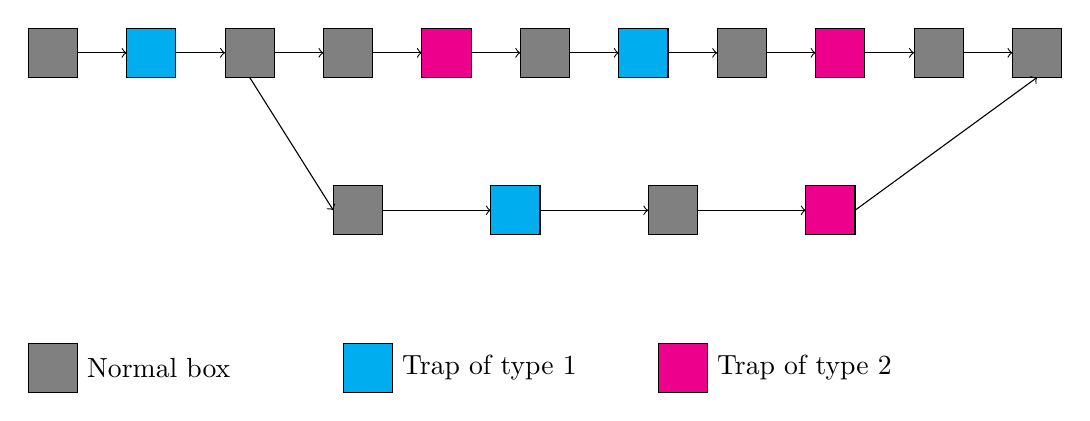
\begin{tikzpicture}[scale=10]
%board = [0,1,0,0,2,0,1,0,2,0,0,1,0,2,0]
\pgfmathsetmacro{\i}{1-1}
\pgfmathsetmacro{\c}{"gray"}
\draw [fill=\c] (2*\i*0.0625,1) rectangle (2*\i*0.0625+0.0625,1-0.0625);
\pgfmathsetmacro{\i}{2-1}
\pgfmathsetmacro{\c}{"cyan"}
\draw [fill=\c] (2*\i*0.0625,1) rectangle (2*\i*0.0625+0.0625,1-0.0625);
\pgfmathsetmacro{\i}{3-1}
\pgfmathsetmacro{\c}{"gray"}
\draw [fill=\c] (2*\i*0.0625,1) rectangle (2*\i*0.0625+0.0625,1-0.0625);
\pgfmathsetmacro{\i}{4-1}
\pgfmathsetmacro{\c}{"gray"}
\draw [fill=\c] (2*\i*0.0625,1) rectangle (2*\i*0.0625+0.0625,1-0.0625);
\pgfmathsetmacro{\i}{5-1}
\pgfmathsetmacro{\c}{"magenta"}
\draw [fill=\c] (2*\i*0.0625,1) rectangle (2*\i*0.0625+0.0625,1-0.0625);
\pgfmathsetmacro{\i}{6-1}
\pgfmathsetmacro{\c}{"gray"}
\draw [fill=\c] (2*\i*0.0625,1) rectangle (2*\i*0.0625+0.0625,1-0.0625);
\pgfmathsetmacro{\i}{7-1}
\pgfmathsetmacro{\c}{"cyan"}
\draw [fill=\c] (2*\i*0.0625,1) rectangle (2*\i*0.0625+0.0625,1-0.0625);
\pgfmathsetmacro{\i}{8-1}
\pgfmathsetmacro{\c}{"gray"}
\draw [fill=\c] (2*\i*0.0625,1) rectangle (2*\i*0.0625+0.0625,1-0.0625);
\pgfmathsetmacro{\i}{9-1}
\pgfmathsetmacro{\c}{"magenta"}
\draw [fill=\c] (2*\i*0.0625,1) rectangle (2*\i*0.0625+0.0625,1-0.0625);
\pgfmathsetmacro{\i}{10-1}
\pgfmathsetmacro{\c}{"gray"}
\draw [fill=\c] (2*\i*0.0625,1) rectangle (2*\i*0.0625+0.0625,1-0.0625);
\pgfmathsetmacro{\i}{11-11}
\pgfmathsetmacro{\c}{"gray"}
\draw [fill=\c] (0.45+\i*0.2,0.8) rectangle (0.45+\i*0.2-0.0625,0.8-0.0625);
\pgfmathsetmacro{\i}{12-11}
\pgfmathsetmacro{\c}{"cyan"}
\draw [fill=\c] (0.45+\i*0.2,0.8) rectangle (0.45+\i*0.2-0.0625,0.8-0.0625);
\pgfmathsetmacro{\i}{13-11}
\pgfmathsetmacro{\c}{"gray"}
\draw [fill=\c] (0.45+\i*0.2,0.8) rectangle (0.45+\i*0.2-0.0625,0.8-0.0625);
\pgfmathsetmacro{\i}{14-11}
\pgfmathsetmacro{\c}{"magenta"}
\draw [fill=\c] (0.45+\i*0.2,0.8) rectangle (0.45+\i*0.2-0.0625,0.8-0.0625);
\pgfmathsetmacro{\i}{15-5}
\pgfmathsetmacro{\c}{"gray"}
\draw [fill=\c] (2*\i*0.0625,1) rectangle (2*\i*0.0625+0.0625,1-0.0625);

\foreach \i in {0,1,...,9}
	\draw [->] (0.0625+2*\i*0.0625,1-0.03125) -- (2*0.0625+2*\i*0.0625,1-0.03125);
\foreach \i in {0,1,2}
	\draw [->] (0.45+\i*0.2,0.8-0.03125) -- (0.45+0.1375+\i*0.2,0.8-0.03125);
\draw [->] (5*0.0625-0.03125,1-0.0625) -- (0.45-0.0625, 0.8-0.03125);
\draw [->] (0.45+0.1375+2*0.2+0.0625,0.8-0.03125) -- (2*10*0.0625+0.0625/2,1-0.0625);

\draw [fill=gray] (0,0.6) rectangle (0.0625, 0.6-0.0625);
\node [right] at (0.0625, 0.6-0.03125) {Normal box};
\draw [fill=cyan] (0.4,0.6) rectangle (0.4 + 0.0625, 0.6-0.0625);
\node [right] at (0.4 + 0.0625, 0.6-0.03125) {Trap of type 1};
\draw [fill=magenta] (0.8,0.6) rectangle (0.8 + 0.0625, 0.6-0.0625);
\node [right] at (0.8 + 0.0625, 0.6-0.03125) {Trap of type 2};
\end{tikzpicture}
\caption{Representation of our board.}
\label{fig:board_unif_low}
\end{figure}
% subsection choosing_the_board (end)

\subsection{Design of the experiments}
Given a particular board configuration, we executed the following three types of experiments : 
\begin{enumerate}
	\item Comparison of simulated and expected cost starting from box 1.
	The simulated cost is the average cost obtained ater a certain number of simulations.
	It is computed for a number of simulations that varies between $10$ and $10^7$. 
	The evolution of this cost is then plotted together with the expected cost obtained by value-iteration.
	\item Comparison of simulated and expected cost starting from each box for a fixed number of simulations.
	\item Comparison of simulated cost using the optimal strategy and some sub-optimal strategies. 
	Here, the evolution of the average cost  with the number of simulations are displayed for each strategy on the same graph.
\end{enumerate}
The following sections contain the results for each experiments and comments.

\subsection{Simulated and expected cost from box 1}

\begin{figure}[H]
\centering
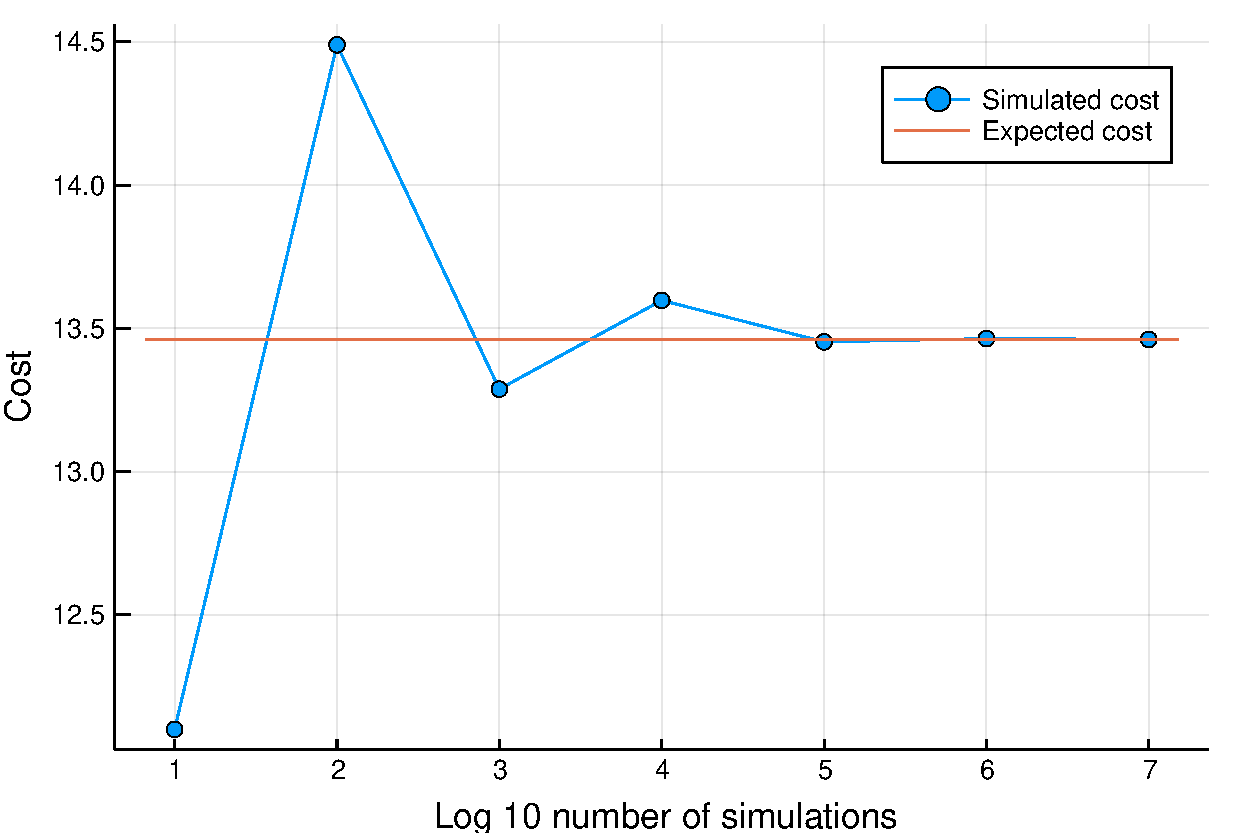
\includegraphics[scale=0.41]{../img/board_unif_low/cost_iterations_log.pdf}
\caption{Evolution of the simulated cost with the number of simulations. The horizontal line represent the expected cost computed with the value-iteration algorithm.}
\label{fig:cost_iterations_log}
\end{figure}


% section results (end)